% ==== ページ関連設定
\documentclass[b5j, twoside, 9pt]{ltjsbook}
\usepackage{mybook}

\newcommand{\mybooktitle}   {Arduinoで始めるアセンブリ}
\newcommand{\mybooksubtitle}{アセンブリからマイコンの機能を使う}
\newcommand{\mybookauthor}  {nikachu2012}
\newcommand{\mybookkeywords}{Assembly, Assembler, Arduino, AVR, ATmega328P}


\ifdefined\isPaperPublishing
    % トンボをつける
    %   pdfbox PDF内にデジタルトンボを埋め込む
    \usepackage[pdfbox, tombo]{gentombow}
\else
    % 電子版の場合は表1-4埋め込み用のpdfpagesをインクルード
    \usepackage{pdfpages}
\fi

% トンボをつける
%   pdfbox PDF内にデジタルトンボを埋め込む
% \usepackage[pdfbox]{gentombow}

% 和文にヒラギノ角ゴ ProNを使う
%   deluxe 多ウェイトを使えるようにする
%   expert 仮名が良い感じになる
%   scale  和文/欧文のサイズ=0.92...にする
\usepackage[hiragino-pron, deluxe, expert, match, scale]{luatexja-preset}
% \usepackage[haranoaji, deluxe, expert, match]{luatexja-preset}

% デフォルトフォントをゴシック体に
\renewcommand{\familydefault}{\sfdefault}
\renewcommand{\kanjifamilydefault}{\gtdefault}

% 和文明朝フォント
\setmainfont{Hiragino Mincho ProN}
% 欧文フォント
\setsansfont{Helvetica Neue}
% 等幅フォント
\setmonofont{Roboto Mono}

% ==== 各種パッケージ
\usepackage{graphicx} % 画像の挿入
\usepackage{amsmath}  % 数式系
\usepackage{xcolor}   % 色
\usepackage{hyperref} % ハイパーリンク
\usepackage{tcolorbox} % ソースコードの枠
\tcbuselibrary{breakable} % tcolorbox内でページまたぎを有効にする
\usepackage{subfiles} % ファイル分割
\usepackage{wrapfig} % 画像を回り込ませる
\usepackage{here}    % 位置指定Hを追加する
\usepackage{enumitem} % itemizeやdescriptionの拡張
\usepackage{ulem} % 打消し線など

\graphicspath{{image/}}

% ==== Hyperref
\usepackage{hyperref} % ハイパーリンク hyperrefは最後にインポート必ず
\hypersetup{%
    bookmarksnumbered=true,%
    bookmarkstype=toc,%
    pdftitle={\mybooktitle},%
    pdfsubject={\mybooksubtitle},%
    pdfauthor={\mybookauthor},%
    pdfkeywords={\mybookkeywords},%
    hidelinks%
}

% メインカラーを定義
\renewcommand{\mybookmaincolor}{\color[cmyk]{0.80, 0.35, 0.22, 0}}

\begin{document}
\ifdefined\isPaperPublishing\else
    % 表１を挿入
    \thispdfpagelabel{表1}
    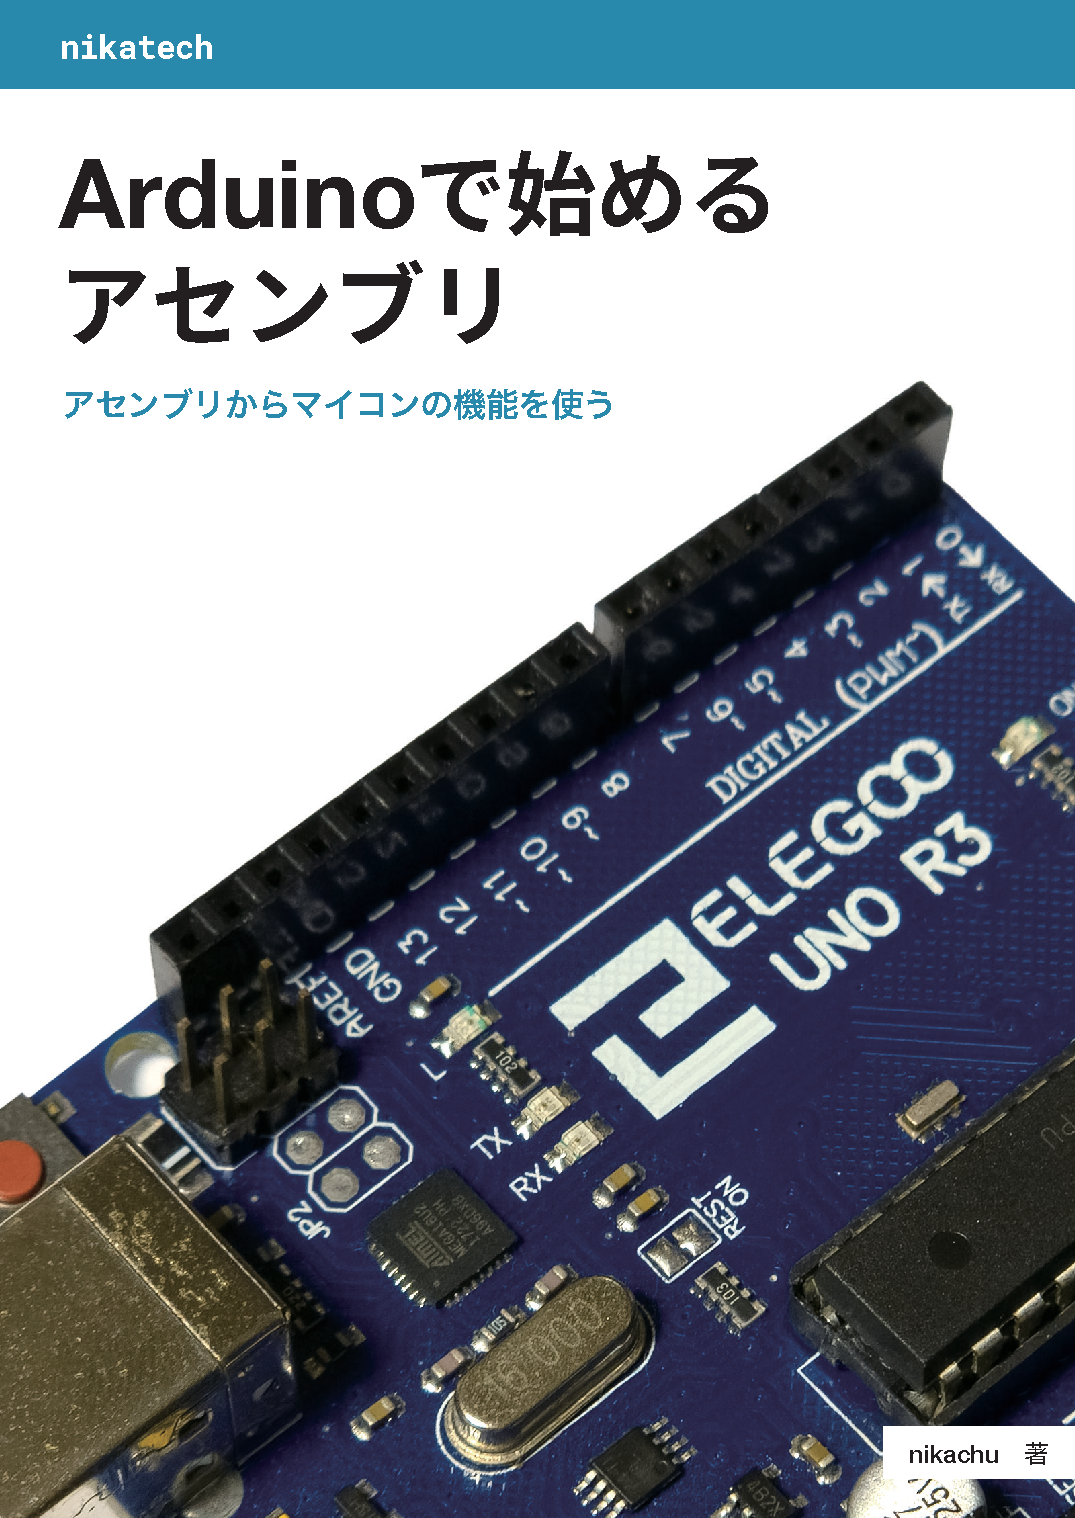
\includepdf[]{_title/avrasm_表1.pdf}
    \newpage
    % 表2を挿入
    \thispdfpagelabel{表2}
    \thispagestyle{empty}
    \null
    \newpage
    \setcounter{page}{1} % ページ変数を1に
\fi

\title{\mybooktitle}
\author{\mybookauthor}
\date{}
\maketitle

\null
\vfill

\begin{tcolorbox}[breakable, colframe=black, sharp corners]
    本書のサポートページは、以下のURLから閲覧することができます。
    \begin{center}
        \url{https://nikatech.nikachu.net/item/avrasm}
    \end{center}
\end{tcolorbox}


\begin{tcolorbox}[breakable, colframe=black, sharp corners]
    本文中にある会社名、製品名は各社の登録商標である可能性があります。本文では\copyright などの表記は行っていません。
\end{tcolorbox}

\begin{tcolorbox}[breakable, colframe=black, sharp corners]
    この本を使用して発生したいかなる損害について筆者、販売員は一切責任を負いません。予めご了承ください。
\end{tcolorbox}

\vspace*{10mm}

%　 はじめに
\subfile{_preface.tex}

\tableofcontents


\chapter{チャプター}

本稿では、沼津高専\footnote{独立行政法人\;国立高等専門学校機構\;沼津工業高等専門学校}にて全学生に配布されている学生証についてできるだけ開設する。また、学生証を用いたシステム開発の手助け等を目的として執筆している。%

\section{セクション}

本物は見せられないので忠実に再現した画像を用いる.\par

% $255_{10}=$ \directlua{toHexString(2147483648)}\par

\begin{figure}[htbp]
    \centering
    \caption{画像サンプル}
    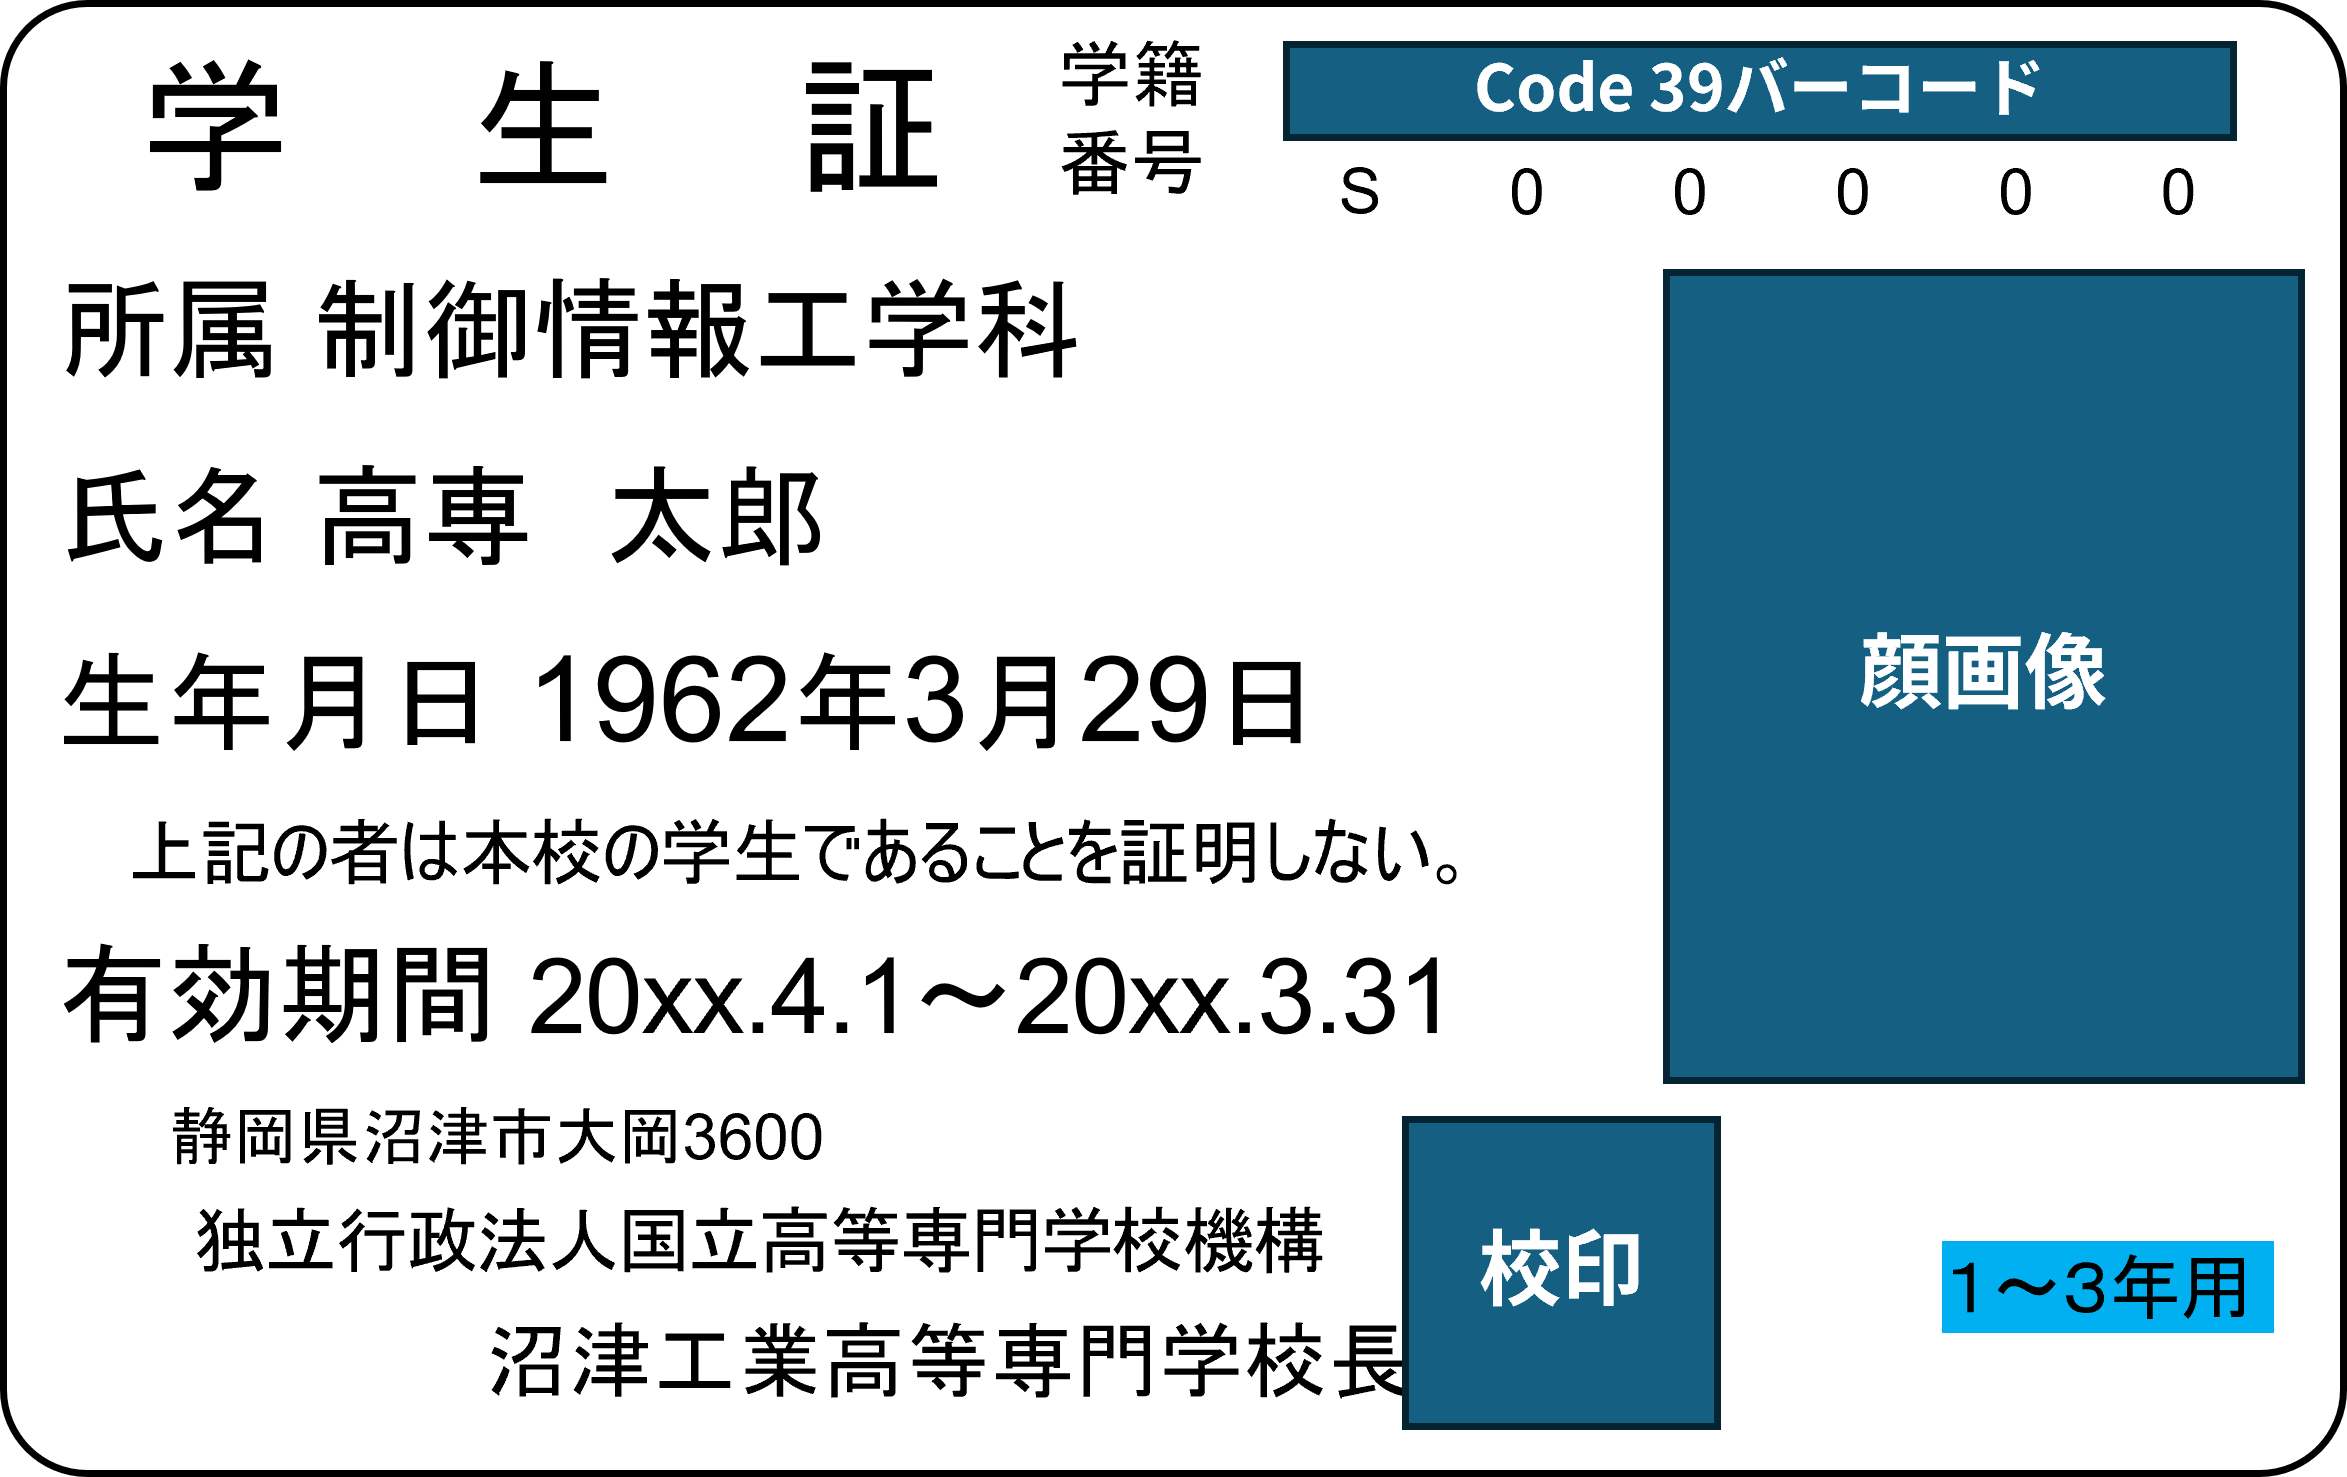
\includegraphics[width=85.60truemm]{image/front.png}
    \label{fig:gakusei_front}
\end{figure}

フォントは数字部分はArial, 日本語部分はMS UI Gothicが使われていると思われる.

サイズはクレジットカードなどと同じ53.98x85.60mmとなっている.
\LaTeX が仕事をしていれば実寸大になっているはず.


\begin{itemize}
    \item 機械工学科
          \begin{itemize}
              \item 電気電子工学科
                    \begin{itemize}
                        \item 電子制御工学科
                              \begin{itemize}
                                  \item 制御情報工学科
                                  \item 物質工学科
                              \end{itemize}
                    \end{itemize}
          \end{itemize}
\end{itemize}

定積分の定義は以下のようになります多分。

\begin{equation*}
    \int_a^b f(x) \,dx = \lim_{n \to \infty} \sum_{i=1}^{n} f(x_i^*) \Delta x_i
\end{equation*}

\clearpage

\subsection{サブセクション}

\subsubsection{サブサブセクション}

ここに \texttt{inline code} が入ります。
ここに \texttt{inline code}\ が入ります。

以下がソースコードです。

\begin{sourcecode}{これがキャプション}
int main(void)
{
    // 日本語だよ
    // This is comment!
    printf("Hello world!");
}
\end{sourcecode}

以下のように書くとファイルからソースコードを表示できます。
\begin{sourcecode}
\begin{codebox}
    \lstinputlisting[]{source/serial_out.asm}
\end{codebox}
\end{sourcecode}

\clearpage

これがコールアウトです。
\begin{note}
    \texttt{\$ npm run dev}を実行しないと、処理が開始されません。必ず実行するようにしてください。
\end{note}

\begin{warn}
    \texttt{\$ npm run dev}を実行しないと、処理が開始されません。必ず実行するようにしてください。
\end{warn}

\begin{caution}
    \texttt{\$ npm run dev}を実行しないと、処理が開始されません。必ず実行するようにしてください。
\end{caution}

\begin{description}
    \item[これがdescriptionのタイトル]
    これが内容
\end{description}

\appendix

\chapter{彼女作るンゴ}

\section{結論}

無理。

\newpage

% 終わりに
\subfile{_afterword.tex}

% 奥付
\subfile{_colophon.tex}

\ifdefined\isPaperPublishing\else
    \newpage
    % 表3の挿入
    \thispdfpagelabel{表3}
    \thispagestyle{empty}
    \null
    \newpage
    % 表4を挿入
    \thispdfpagelabel{表4}
    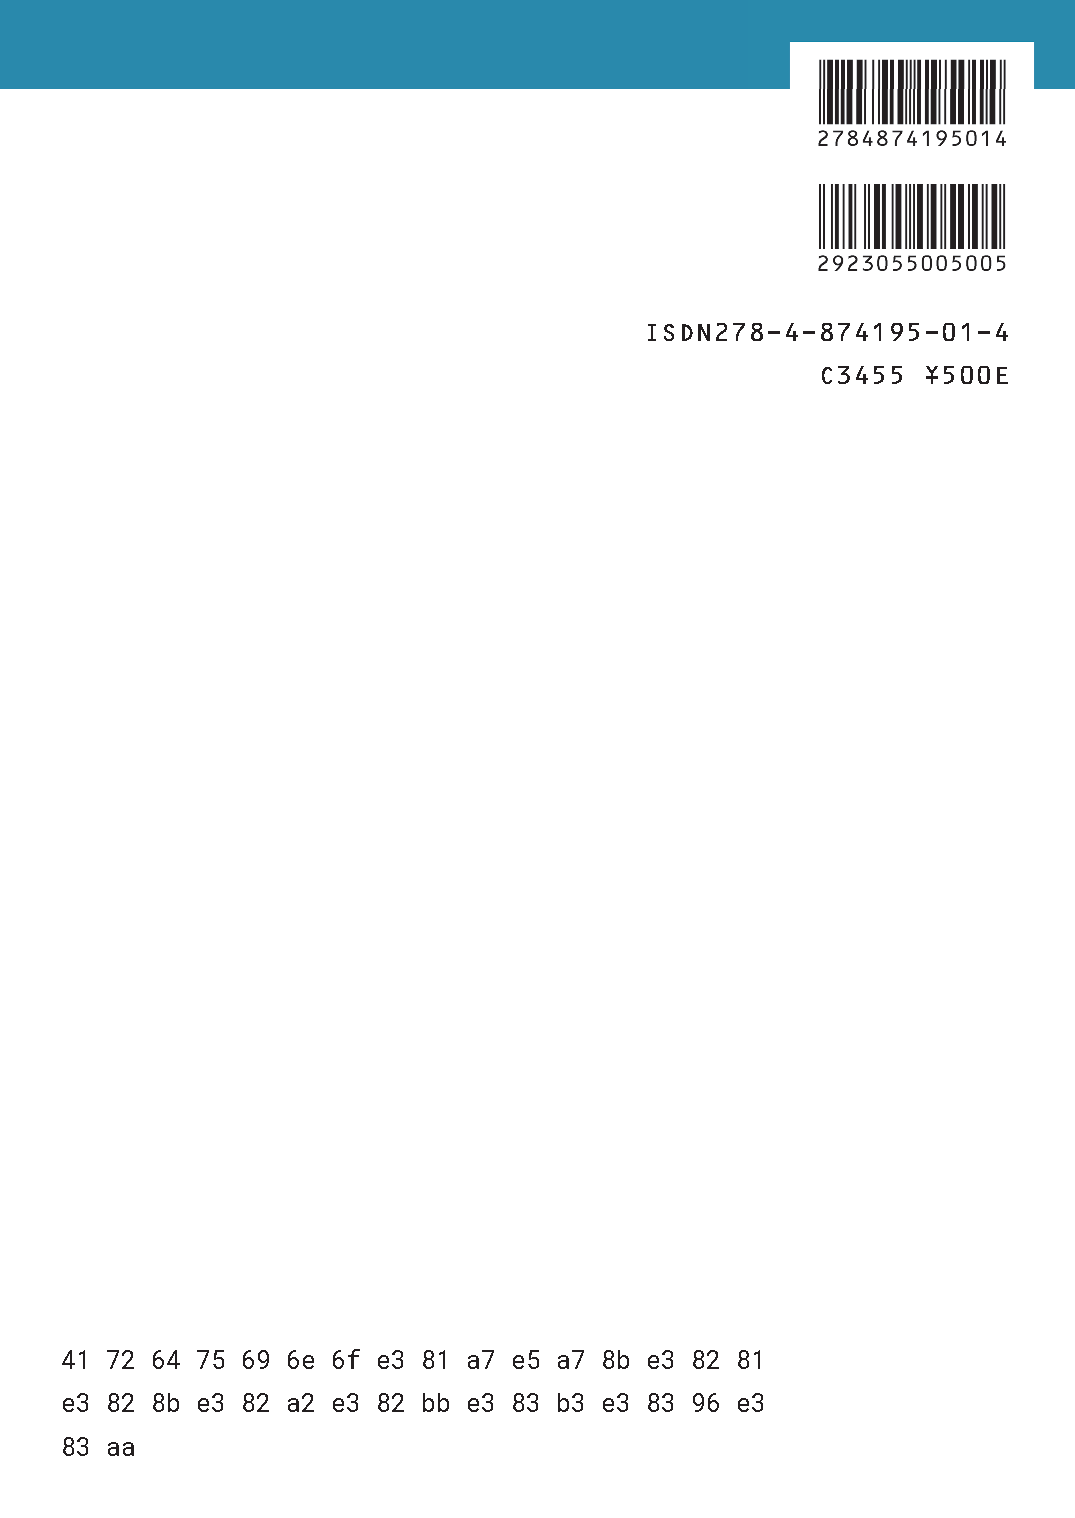
\includepdf[]{_title/avrasm_表4.pdf}
\fi


\end{document}


